\documentclass[letterpaper,11pt]{article}
\pdfoutput=1

\usepackage[utf8]{inputenc}

\usepackage{jheppub,multirow, amsthm,mathrsfs,xspace,xcolor,float,color,siunitx,comment}
\usepackage[caption=false]{subfig}
\usepackage[countmax]{subfloat}

\newcommand{\R}{\mathbb{R}}
\newtheorem{theorem}{Theorem}
\providecommand{\href}[2]{#2}

\definecolor{darkred}{rgb}{0.5,0.0,0.0}
\definecolor{darkblue}{rgb}{0.0,0.0,0.9}
\definecolor{darkerblue}{rgb}{0.0,0.0,0.5}
\definecolor{darkgreen}{rgb}{0.0,0.5,0.0}
\definecolor{black}{rgb}{0.0,0.0,0.0}
\definecolor{brown}{rgb}{0.6,0.4,0.2}
\newcommand{\red}{\color{darkred}}
\newcommand{\blue}{\color{darkblue}}
\newcommand{\green}{\color{darkgreen}}
\newcommand{\black}{\color{black}}

\DeclareRobustCommand{\Sec}[1]{Sec.~\ref{#1}}
\DeclareRobustCommand{\Secs}[2]{Secs.~\ref{#1} and \ref{#2}}
\DeclareRobustCommand{\Secss}[3]{Secs.~\ref{#1}, \ref{#2} and \ref{#3}}
\DeclareRobustCommand{\App}[1]{App.~\ref{#1}}
\DeclareRobustCommand{\Tab}[1]{Table~\ref{#1}}
\DeclareRobustCommand{\Tabs}[2]{Tables~\ref{#1} and \ref{#2}}
\DeclareRobustCommand{\Fig}[1]{Fig.~\ref{#1}}
\DeclareRobustCommand{\Figs}[2]{Figs.~\ref{#1} and \ref{#2}}
\DeclareRobustCommand{\Figss}[3]{Figs.~\ref{#1}, \ref{#2} and \ref{#3}}
\DeclareRobustCommand{\Eq}[1]{Eq.~(\ref{#1})}
\DeclareRobustCommand{\Eqs}[2]{Eqs.~(\ref{#1}) and (\ref{#2})}
\DeclareRobustCommand{\Ref}[1]{Ref.~\cite{#1}}
\DeclareRobustCommand{\Refs}[1]{Refs.~\cite{#1}}

\newcommand{\ijm}[1]{\marginpar{\raggedright\scriptsize\textbf{\textcolor{red}{ijm}}}  \textbf{\textcolor{red}{(#1 --ijm)}}}

%Change float fractions
\renewcommand{\floatpagefraction}{0.50}

\widowpenalty10000
\clubpenalty10000

\title{Ending the Alphabet of Quark/Gluon Discriminants}

\preprint{ 
\begin{flushright}
MIT--CTP xyz
 \end{flushright}}

\author[a]{Eric M. Metodiev,}
\author[b,c]{Ian Moult}
\author[d]{and Benjamin Nachman}

\affiliation[a]{Center for Theoretical Physics, Massachusetts Institute of Technology, Cambridge, MA 02139, USA}
\affiliation[b]{Berkeley Center for Theoretical Physics, University of California, Berkeley, CA 94720, USA}
\affiliation[c]{Theoretical Physics Group, Lawrence Berkeley National Laboratory, Berkeley, CA 94720, USA}
\affiliation[d]{Physics Division, Lawrence Berkeley National Laboratory, Berkeley, CA 94720, USA}


\emailAdd{metodiev@mit.edu}
\emailAdd{ianmoult@lbl.gov}
\emailAdd{bpnachman@lbl.gov}


\abstract{
The radiation pattern within high energy jets contains a wealth of information about the originating particle.
%
Numerous techniques have been developed based on qualitative features of jet substructure, with the resulting observables calculated to high perturbative accuracy in many cases.
%
At the same time, there have been many attempts to fully exploit the jet radiation pattern using tools from statistics and machine learning.
%
We propose a new approach that combines a deep analytic understanding of jet substructure with the optimality motivation from machine learning and statistics.
%
After specifying an approximation to the full emission phase space, the optimal observable is calculated exactly.
%
This procedure is demonstrated for the case of quark and gluons jets in the leading logarithmic and modified leading logarithmic approximation, where we prove that linear combinations of weighted multiplicity is the optimal observable.
%
In addition to providing a new and powerful framework for systematically improving jet substructure observables, the specific quark versus gluon jet tagging observable is demonstrated to improve upon the performance of existing substructure observable approaches.
}


\begin{document} 
\maketitle
\flushbottom





%%%%%%%%%%%%%%%%%%%
\section{Introduction}
\label{sec:intro}
%%%%%%%%%%%%%%%%%%%






Collimated sprays of particles initiated by high energy quarks and gluons are a ubiquitous feature of collisions at the Large Hadron Collider (LHC).
%
The radiation pattern within these \textit{jets} contains a wealth of information about the originating particle.
%
Since the start of the LHC, there has been a revolution in jet substructure that has resulted in many tools developed to tag the origin of a jet~\cite{Butterworth:2008iy,Abdesselam:2010pt,Altheimer:2012mn,Altheimer:2013yza,Adams:2015hiv}.
%
These tools have significantly extended the reach of searches for physical phenomena beyond the Standard Model (SM) as well precision measurements in the SM.
%


The most successful and widely used techniques apply to situations where the radiation pattern within the jet exhibits hierarchical structures. This occurs in many cases of relevance, such as $n$-prong tagging for identifying hadronically decaying bosons or top quarks. In such cases, power counting \cite{Larkoski:2014gra} can be used to identify optimal observables as an expansion in the hierarchical parameter. For instance, the ATLAS collaboration two-prong tagger default $D_2$ \cite{Larkoski:2014gra}, and the CMS collaboration two-prong tagger $N_2$ \cite{Moult:2016cvt} were constructed by power counting. This approach has the advantage that it makes clear the physics identified by the observable.
%
Once motivated and defined, many of the state-of-the-art observables have been calculated with high formal precision~\cite{Larkoski:2017iuy}.  However, this approach fails when there does not exist a clear expansion parameter. One such case is quark/gluon tagging, which despite having significant potential applications at the LHC, has achieved limit theory success due to the lack of a systematic approach to the construction of observables.


Modern machine learning has revolutionized the way classification techniques are optimized in many fields.
%
Deep neural networks trained on a low-level representation of the full radiation pattern inside jets have been found to outperform observables simple physics motivated features.
%
For a review of machine learning techniques in jet physics, see \Ref{Larkoski:2017jix}.
%
A key challenge with these machine learning tools is that they are intractable to understand physically.
%
This has motivated a series of proposals to use physically-motivated bases of high-level features~\cite{Datta:2017rhs,Datta:2017lxt,Luo:2017ncs,Komiske:2017aww}.
%
These proposals guarantee important properties for classification, such as completeness or linearity, but nonetheless still may not result in sufficient analytic control over the final classifier to be understood simply.
%
While a first-principles understanding of a classifier is not strictly required for its performance, it can add robustness when the technique is applied beyond its training domain and furthermore can lead to a deeper understanding of the underlying physics.

In this paper, we introduce a new approach that combines the benefits of both first-principles techniques and statistical machine learning algorithms.
%
First, an approximation of the full emission phase space is constructed.
%
A well-known theorem due to Neyman and Pearson~\cite{neyman1933ix} states that the optimal classifier for distinguishing two classes is a threshold on the ratio of the class probability densities (likelihood ratio).
%
With a description of the full emission phase space for two classes, one can take the full ratio and reorganize terms to arrive at an analytic prediction for the optimal classifier. In this sense it is similar to shower deconstruction~\cite{Soper:2012pb}.
%
This procedure is systematically improvable as the approximation to the full phase space is improved. Unlike the power counting approach, this approach does not rely on the existence of a small parameter. As compared to standard ML techniques, since it is based on understanding the analytic approximation used to derive the likelihood, it makes clear what physics is being exploited, and furthermore, what must be exploited to achieve improved performance


We will apply this approach to the case of quark/gluon discrimination, which has so far resisted organizing principles. We will prove that in the approximation of eikonal splitting functions, the optimal observable is multiplicity. We then extend this to modified leading logarithmic accuracy, and prove that the optimal observable is a linear combination of weighted multiplicities. Using this, we introduce a new quark/gluon discriminant, which we find in parton shower simulations outperforms standard observables.

This paper is organized as follows. In \Sec{sec:structure} we provide a review of the structure of quark and gluon jets. Section~\ref{sec:squirrel} describes an explicit example of an optimal classifier for quark versus gluon jet tagging with leading logarithm (LL) and then at next-to-leading logarithm (NLL) precision.  The performance of the resulting tagger is shown in Sec.~\ref{sec:squirrelemperical} using parton shower (PS) Monte Carlo (MC) simulations.  Finally, Sec.~\ref{sec:conc} discusses how this approach could be extended to other tagging problems before concluding.




%%%%%%%%%%%%%%%%%%%%%%%%%%%%%%%%%
\section{Reviewing the Structure of Quark and Gluon Jets}
\label{sec:structure}
%%%%%%%%%%%%%%%%%%%%%%%%%%%%%%%%%

We begin by analyzing the perturbative structure of a jet sourced by a hard parton radiating massless gauge bosons (the radiation of fermions will be adressed later). Here we will restrict ourselves to LL or MLL, where we can use the splitting functions. While this is very well understood, here we present what is perhaps a different perspective that proves particularly useful for understanding quark vs. gluon discrimination.\footnote{This perspective has been beautifully advocated for the simplification of the higher order splitting functions in \cite{Dokshitzer:2005bf,Dokshitzer:2006nm,Beccaria:2007bb}.}


Although we will be focused on the physically realized case of QCD, it is interesting to view the problem more generally. We consider the splitting function for the radiation of a massless gauge boson
\begin{align}\label{eq:split_general}
=4C_i \frac{\alpha}{4\pi} \left(\frac{x}{1-x}+(1-x) g_i(x)   \right)\,, \qquad \left\{ \begin{array}{c}g_\phi=0 \\ g_\lambda=\frac{1}{2} \\g_V=x+\frac{1}{x} \end{array} \right. \,.
\end{align}
\ijm{write it in the symmetrized form for the gluon}
The function $g_i(x)$ satisfies the condition that it has a regular Taylor series expansion about $x=1$. Here we see that the splitting probability depends on the parton species through two factors: the Casimir $C_i$ which describes the color charge of the particle, and the function $g_i(x)$.

In the $x\to 1$ limit, in which the emitted radiation is soft, and which is enhanced by the soft singularity, the splitting function exhibits a universal form, depending only on the color factor, $C_i$, which to be explicit, are
\begin{align}
C_F=\frac{N^2-1}{2N}\to \frac{4}{3}\,, \qquad C_A=N\to 3\,.
\end{align}
The coefficient appearing in the splitting function is simply the one-loop cusp anomalous dimension. The result in this limit is of course simply the classical result for radiation in the eikonal limit \cite{Levy:1969cr}. \footnote{We wish to emphasize that the leading double logarithmic Sudakov is classical.} The classical result is (as it must be) independent of the spin of the emitting parton. In this limit, there is no information contained in the structure of the radiation within the jet. The only information is contained in the quantity of radiation (multiplicity). We will prove this rigorously in \Sec{sec:squirrel}.

The second factor $g_i(x)$ in the splitting function depends on the nature of the emitted. It's contribution to the splitting function is suppressed by two powers of the $(1-x)$. This is guaranteed by the Low-Burnett-Kroll theorem \cite{Low:1958sn,Burnett:1967km,DelDuca:1990gz} describing the soft limits of gauge theories.\footnote{In this case the LBK theorem is applied after taking the collinear limit.} As expected, it vanishes for a scalar, which has no structure beyond its color.


Having written the splitting functions in the above form makes abundantly clear the difficulty for quark gluon discrimination: the structure of a jet is dominated by its classical result, and therefore depends only on the color charge. Futhermore, we note an amusing difference. Expanding the $g_i$ in $(1-x)$, we have
\begin{align}
g_\phi=0\,, \qquad g_\lambda=\frac{1}{2}\,, \qquad g_V=\frac{1}{2}+\frac{1}{4}(1-x)^2+\cdots\,.
\end{align}
Therefore, the difference between a quark and a gluon is in fact more suppressed than it needs to be.


%The leading divergence in the limit that the emitted gauge boson is soft is the classical result.\ijm{The LL Sudakov is a purely classical result.} As such, it is independent of the spin structure of the emitting parton, and depends only on its color charge. (The coefficient is simply the one-loop cusp anomalous dimension). The corrections which depend on the spin structure of the emitting parton are down by two powers of $(1-x)$. This is guaranteed by the LBK theorem applied after first taking the collinear limit. 










We note that in QCD, there is an additional distinction between quarks and gluons, namely that gluons can split into a $q\bar q$ pair,
\begin{align}
P_{g\to q\bar q}(z) & = \frac{n_f T_R}{2C_A}[z^2 + (1-z)^2].
\end{align}
This splitting does not obey the LBK theorem,\footnote{See \cite{Moult:2016fqy,Boughezal:2016zws,Moult:2017jsg,Boughezal:2018mvf,Moult:2018jjd} for a discussion.} and is down only by a single power of $z$.


\ijm{can one argue something about the behavior of the fragmentation function}









%%%%%%%%%%%%%%%%%%%%%%%%%%%%%%%%%
\section{Quark and Gluon Jet Likelihoods}
\label{sec:squirrel}
%%%%%%%%%%%%%%%%%%%%%%%%%%%%%%%%%

In this section we introduce an approach which allows us to prove the optimality of quark/gluon discriminants. This approach consists of analyzing the likelihood function of the jet radiation at a given accuracy. The Neyman-Pearson Lemma~\cite{neyman1933ix} then states that the optimal classifier for distinguishing two classes is a threshold on the ratio of the class probability densities (likelihood ratio).  We believe, however, that this approach is more general, and it would be interesting to apply it to other cases in jet substructure.

\ijm{make some blab about power counting and having a small parameter to expand in}\cite{Larkoski:2014gra}\cite{Moult:2016cvt}\cite{Larkoski:2014zma}


What this approach allows one to do, is to work in some approximation for the likelihood distribution of quarks and gluons. e.g. eikonal approximation, independent emission, etc. We can then analyze this likelihood using ML or information theoretic techniques, to prove results about the optimal observables. These results will then apply to any observables that can be computed at a given accuracy from this likelihood. Since we will always work in some approximation for the likelihood, one can always come up with observables that can evade the proven results, if they cannot be correctly computed from this approximation. However, we view this as a virtue, as it shows how the proven theorems can be evaded.


%%%%%%%%%%%%%%%%%%%%%%%%%%%%%%%%%
\subsection{Analysis in the Eikonal Limit}\label{sec:eik}
%%%%%%%%%%%%%%%%%%%%%%%%%%%%%%%%%

We begin by considering the optimal quark/gluon discriminant in the eikonal limit. We define the eikonal limit as independent emissions with the universal part of the splitting functions
\begin{equation}
\label{eq:LLemit}
dP_{i\to i g}(z,\theta) = \frac{2 \alpha_s C_i}{\pi} \frac{dz}{z}\frac{d\theta}{\theta},
\end{equation}
namely the eikonal factor.

Before proceeding, we would like to clarify a number of issues related to our referring to this as the eikonal, or classical eikonal limit. Another name which could be used is the LL limit. We wish to avoid this language, since it is best defined when their is an observable of interest. While it is of course true that for Sudakov type observables, the above will generate the leading logarithms, it is straightforward to identify IRC safe observables (even those that probe only two particle correlations) for which the leading logarithm will not be produced by the above approximated splitting function. 

Since we have shown that splitting function is identical in this limit for all partons (up to the color factor), we should be able to prove that multiplicity is the optimal observable.

To prove this, we consider the quark/gluon log likelihood $L_{q/g}$ for radiating a collection of gluons\footnote{Here we use the well known fact that there is a probabilistic interpretation for the twist two splitting functions. This, however, should not be taken for granted, and indeed such a probabilistic interpretation fails at higher twist \cite{Jaffe:1982pm}.} with $\{(z_n,\theta_n)\}_{n=1}^M$ 
\begin{equation}
\text{JL}^\text{LL} \equiv\ln L_{q/g}^\text{LL} = \sum_{n=1}^M \ln \frac{dP_{q\to qg}(z_n,\theta_n)}{dP_{g\to gg}(z_n,\theta_n)} = \ln \frac{C_F}{C_A} \sum_{n=1}^M 1 = M \ln \frac{C_F}{C_A}.
\end{equation}
Here $M$ is simply the multiplicity, and so by the Neyman-Pearson Lemma~\cite{neyman1933ix}, the optimal observable at this level of accuracy is the multiplicity. Experimentally the multiplicity is indeed found to behave well, however, we are now able to prove this. In hindsight, this is a completely obvious, and follows simply from the universal nature of soft emissions in gauge theory, or in other words, the classical structure of the jet.  We also note that the above result holds regardless of whether the coupling is taken to be running or not, since it cancels out. 

We therefore state our first result:

\vspace{1cm}
{\bf Theorem I:} For an observable whose LL result can be computed using the eikonal splitting functions of \Eq{eq:LLemit} in the independent emission approximation (with or without running coupling), this LL result can not achieve better quark/gluon discrimination than multiplicity.
\vspace{1cm}


We note that this behavior is true for a very wide class of observables, including standard Sudakov observables, Sudakov observables that have been soft dropped \cite{Larkoski:2014wba}, groomed multiplicity \cite{Frye:2017yrw}.

In addition to showing that multiplicity is optimal, we can in fact derive its probability distribution. Since the sum of Poissonians is Poissonian, so we can immediately read off
\begin{equation}
p^\text{LL}_i(M) = \text{Pois}\left[\int \frac{dz}{z} \int \frac{d\theta}{\theta}\, \frac{2\alpha_s C_i}{\pi} \Theta(z,\theta)\right]\,.
\end{equation}
Poisson observables were emphasized in
\cite{Frye:2017yrw}

A simple way of visualizing this proof is in the Lund plane shown in \Fig{fig:lundschematic}. In the eikonal limit of the splitting functions, emissions are uniformly distributed in the Lund plane. We can therefore tesselate some perturbative region of the Lund plane using triangles. The probability for $n$ emissions in a given triangle is then Poisson distributed with the splitting function
\begin{align}
\Pr(n_i=n)=\frac{\lambda^n e^{-\lambda}}{n!}\,, \qquad \lambda=\frac{2\alpha_s C_i \Delta}{\pi}\,,
\end{align}
due to the assumption of independent emissions, we then have
\begin{align}
{\Pr}_i(n_1, n_2, \cdots, n_N)=\prod\limits_{j=1}^N \frac{\lambda_i^{n_j} e^{-\lambda_i}}{n_j!}\,.
\end{align}
The optimal quark/gluon discriminant is then
\begin{align}
\log \left(  f(n_1, \cdots, n_N) \right)  =   \log \left( \frac{{\Pr}_q(n_1, \cdots, n_N)}{{\Pr}_g(n_1, \cdots, n_N)} \right) =\sum\limits_{j=1}^N n_j \log\left(\frac{C_q}{C_g}  \right)\,.
\end{align}
We can take the $\Delta\to 0$ limit. This is again simply the multiplicity. 

This version of the proof makes clear that we can apply a cutoff and only consider the likelihood function in the perturbative regime.

\ijm{discussion about NP and soft drop mimics LL structure of the shower.}

\ijm{This also makes clear that one can apply an NP cut, and it still holds}

\begin{figure}[t]
\centering
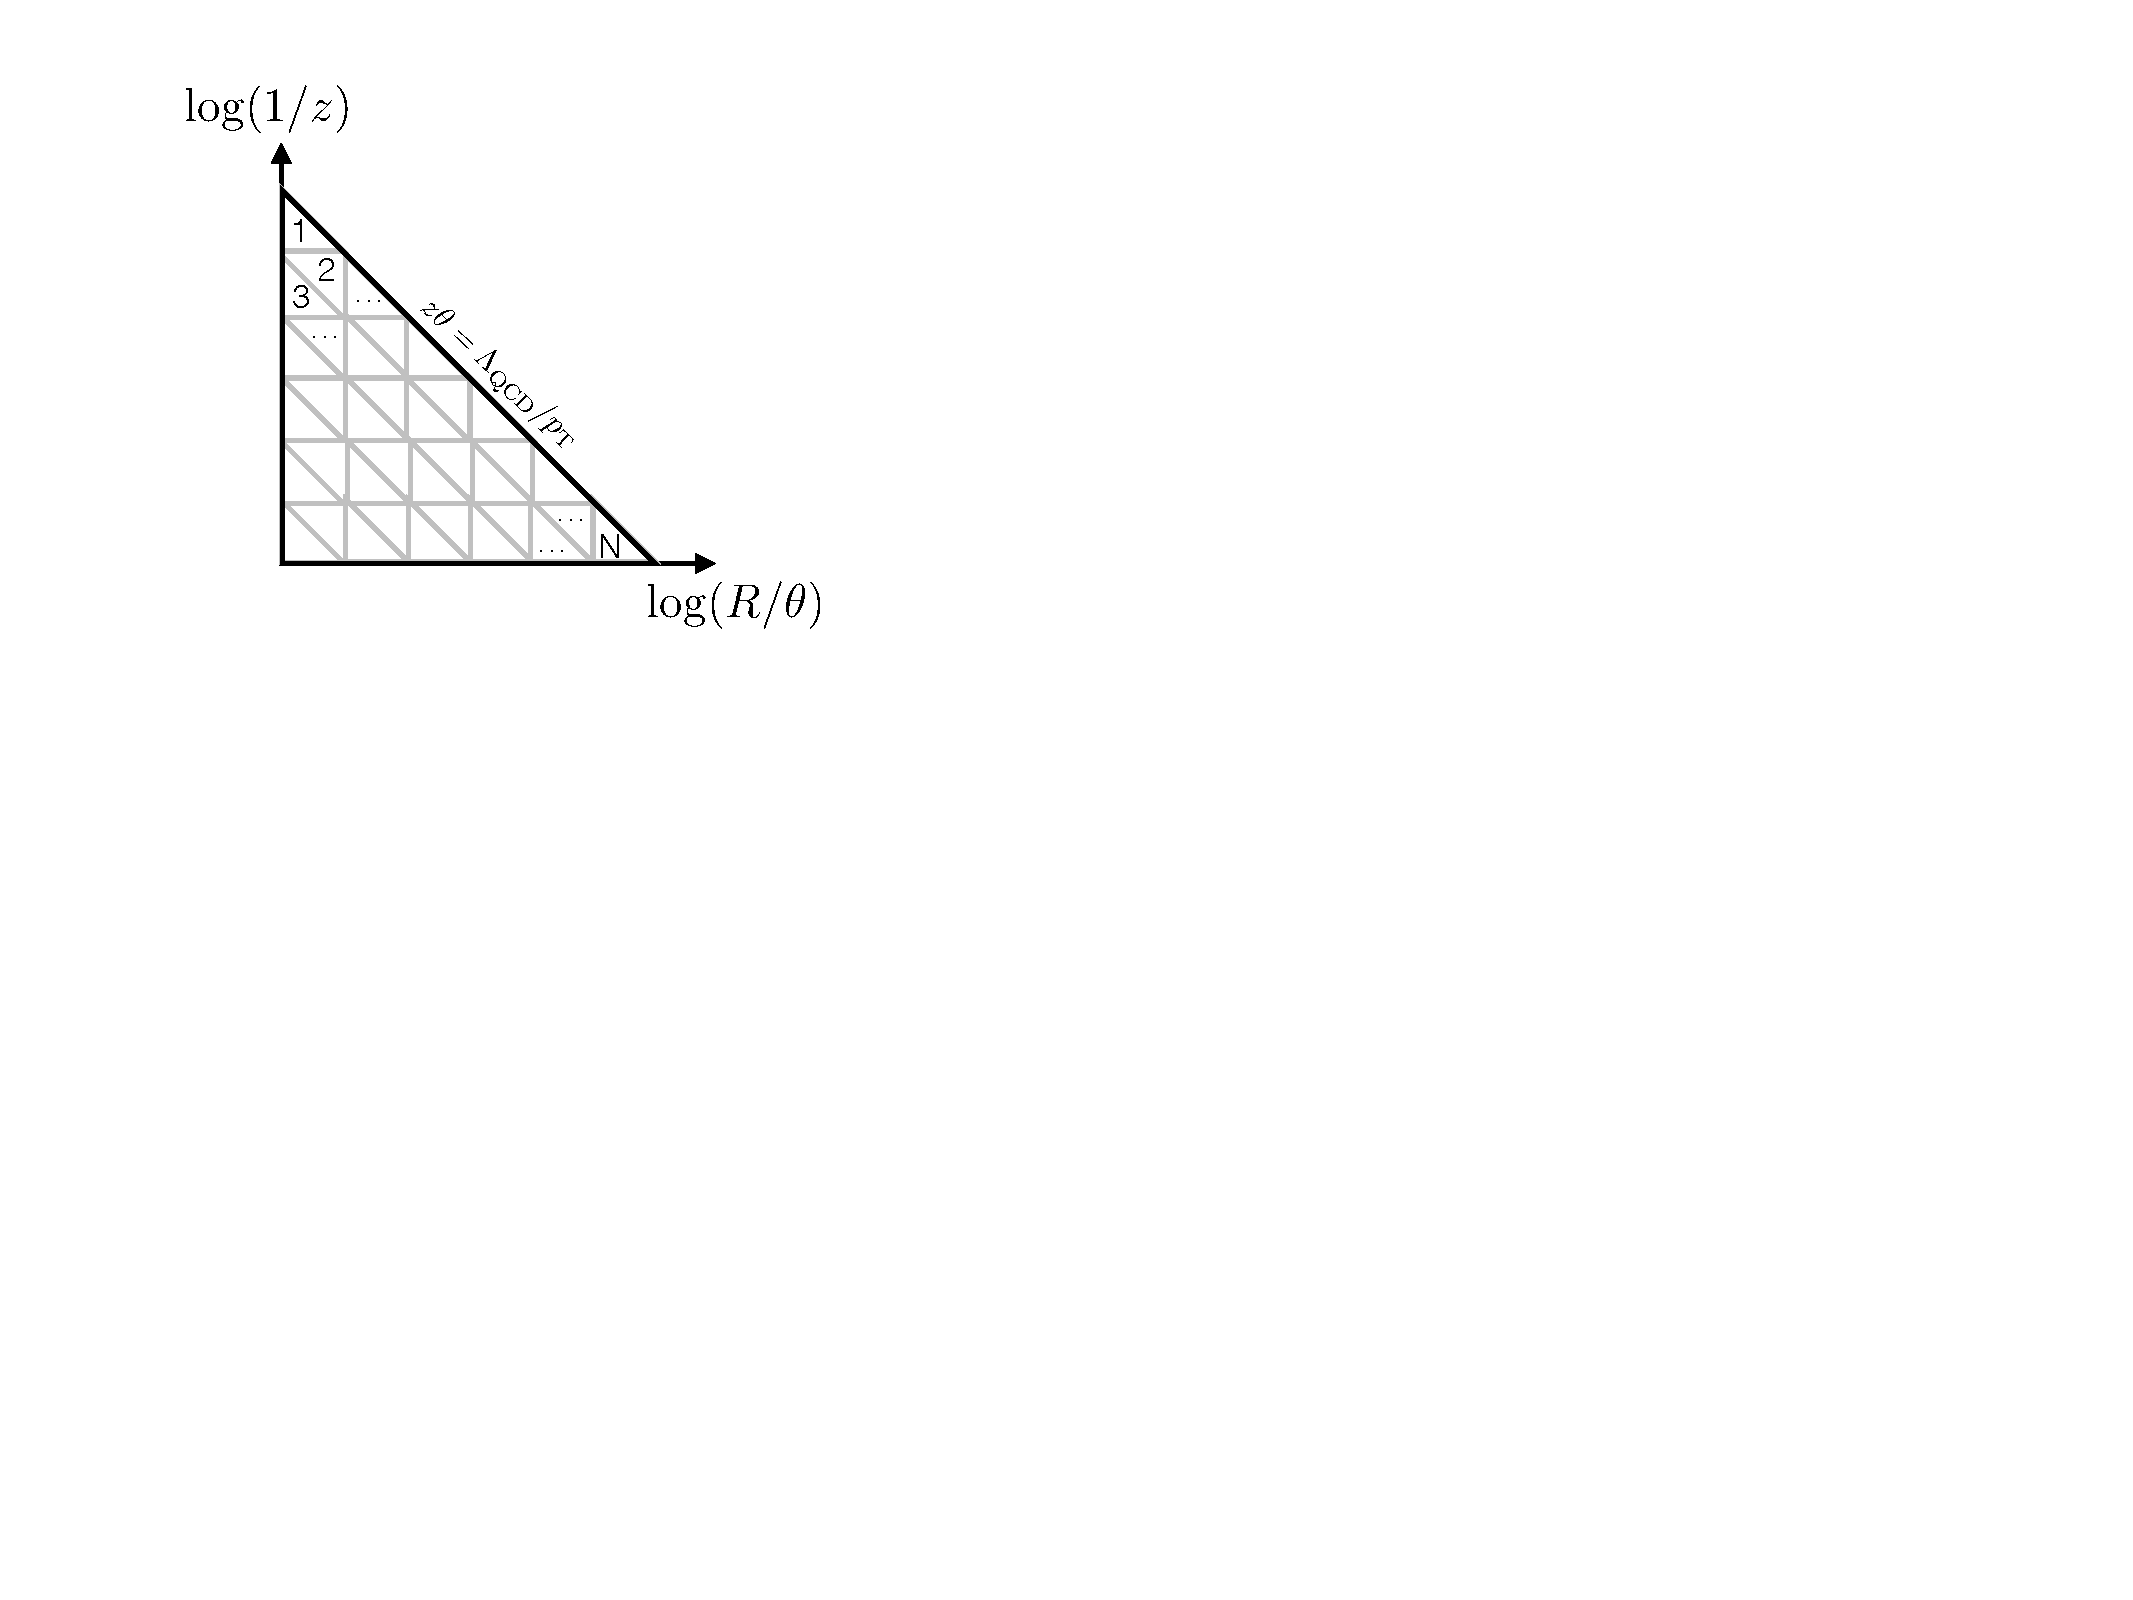
\includegraphics[width=0.5\textwidth]{figures/LundPlaneSchematic.pdf}
\caption{A tiled version of the Lund plane where each of the $N$ triangles has the same area.  The non-perturbative regime is defined by $z\theta>\Lambda_\text{QCD}/p_\text{T}$.}
\label{fig:lundschematic}
\end{figure}


%%%%%%%%%%%%%%%%%%%%%%%%%%%%%%%
\subsection{Modified Leading Logarithmic Analysis}
%%%%%%%%%%%%%%%%%%%%%%%%%%%%%%%

\ijm{need to define very clearly what we mean by modified leading logarithmic analysis.}

The modified leading logarithmic (MLL) approximation includes the effects of running coupling and subleading terms in the splitting function.
\begin{equation}
\label{eq:LLemit}
dP_{i\to i j}(z,\theta) = \frac{2\alpha_s (z\theta p_T) \, C_i}{\pi} P_{i}(z) dz\,\frac{d\theta}{\theta},
\end{equation}



\begin{equation}
\label{eq:MLLLL}
\text{JL}^\text{MLL} \equiv \ln L_{q/g}^\text{MLL} = \sum_{n=1}^M \ln \frac{dP_{q\to qg}(z_n,\theta_n)}{dP_{g\to gg}(z_n,\theta_n)} = \sum_{n=1}^M\left[\ln \frac{C_F}{C_A} + \ln \frac{P_q(z_n)}{P_g(z_n)} \right].
\end{equation}

Can see at this point that the optimal observable is a linear combination of the weighted multiplicities considered in 

The quark and gluon splitting functions, when summed over final states, become:
\begin{align}
P_q(z) & = \frac{1 + (1 - z)^2}{2z},\\
P_g(z) & = \frac{1 - z}{z} + \frac12 z(1-z) + \frac{n_f T_R}{2C_A}[z^2 + (1-z)^2].
\end{align}
where the $z\leftrightarrow 1-z$ symmetry is used put the gluon singularity entirely at $z\to 0$.


The optimal observable at MLL from \Eq{eq:MLLLL} is independent of the running of the strong coupling constant.
%
The splitting functions influence the optimal observable via the log likelihood ratio $\ln P_q(z)/P_g(z)$
%
Restore perturbative multiplicity as the optimal observable in the soft $z_n\to 0$ limit as quarks and gluons have the same soft singularity so the log splitting function ratio approaches zero.

\begin{align}
\label{eq:optobsMLL}
\text{JL}^\text{MLL} & = \sum_{n=1}^M\left[\ln \frac{C_F}{C_A} + \ln \frac{1+(1-z_n)^2}{(1-z_n)(2 + z_n^2) + \frac{n_f T_R}{C_A}z_n(z_n^2 + (1-z_n)^2)} \right].
\end{align}

\begin{align}
\text{JL}^\text{MLL} &= \sum_{n=1}^{M}\left(\ln \frac{C_F}{C_A} - \frac{n_f T_R}{2C_A} z_n + \frac{n_f T_R (4 C_A + n_F T_R)}{8 C_A^2} z_n^2 + \cdots \right)
\\& = \ln \frac{C_F}{C_A} n^{(\kappa = 0 )} - \frac{n_f T_R}{2C_A} n^{(\kappa = 1)} + \frac{n_f T_R (4 C_A + n_F T_R)}{8 C_A^2} n^{(\kappa = 2)} + \cdots
\end{align}

Consider:
\begin{equation}
\mathcal O =  \ln \frac{C_F}{C_A}n^{(\kappa = 0 )} + A \, n^{(\kappa = 1)} + B \, n^{(\kappa = 2)}
\end{equation}
and let's look at discrimination performance in the $(A,B)$-plane $(-1,1)\times(-1,1)$.

Also, can immediately read off:
\begin{equation}
p^\text{MLL}_i(M) = \text{Pois}\left[\int P_i(z)dz \int \frac{d\theta}{\theta}\, \frac{2\alpha_s(z\theta p_T) C_i}{\pi} \Theta(z,\theta)\right]
\end{equation}


\begin{equation}
n^{(\kappa)} \equiv \sum_{n=1}^M z_n^\kappa.
\end{equation}

Must discuss how well soft drop captures the real shower.

We can therefore extend to our second result:

\vspace{1cm}
{\bf Theorem II:} For an observable whose LL or MLL result can be computed using splitting functions in the independent emission approximation, this result can not achieve better quark/gluon discrimination than a linear combination of weighted multiplicities.
\vspace{1cm}


%%%%%%%%%%%%%%%%%%%
\subsection{Bla: A new observable for Quark vs. Gluon Tagging}
\label{sec:new_obs}
%%%%%%%%%%%%%%%%%%%

This extends to a continuous variable the counting variable of \cite{Frye:2017yrw}.


%%%%%%%%%%%%%%%%%%%
\subsection{Discussion and Extensions}
\label{sec:discuss}
%%%%%%%%%%%%%%%%%%%

can discuss how for these observables, higher orders in $\alpha_s$ the same will mostly apply in soft limit. Casimir scaling holds to at least three loops. Violated at four loops\cite{Armoni:2006ux}\cite{Boels:2017skl}.\cite{Grozin:2017css} \cite{Moch:2017uml} these should be small higher order corrections.

Suggests a different direction one should look directly for observables that cannot be computed in these approximations.

study of observables with more interesting logarithmic structures.

%%%%%%%%%%%%%%%%%%%
\section{Monte Carlo Study}
\label{sec:squirrelemperical}
%%%%%%%%%%%%%%%%%%%

Using our Pythia + DIRE setup, we can do some tests:

\begin{enumerate}
\item Turn off $g\rightarrow qq$ and turn off hadronization (will revise these later).  
\begin{enumerate}
	\item LL and set $C_A=C_F$.  Verify that we can't learn anything useful for q/g.
	\item LL but real $C_A$ and $C_F$.
	\item Same, but MLL (LO splitting functions).  For later - this is the `quantum' component.
	\item Now, tweak the finite parts of LO splitting functions and show that we can predict the optimal observable (even more fun to make the second term dominate over the first so that the best observable is not just multiplicity + $\epsilon$; in particular, can set $C_A=C_F$ but have different subleading terms).
\end{enumerate}
\item For one configuration above, check impact of hadronization and $g\rightarrow qq$.
\end{enumerate}

Some notes: maybe we do this in $e^+e^-$ so we don't have to worry about q/g definitions, etc. or pileup or UE.

%%%%%%%%%%%%%%%%%%%
\section{Conclusions}
\label{sec:conc}
%%%%%%%%%%%%%%%%%%%

In this paper we have presented a new approach to understanding jet substructure observables, analyzing their likelihood function at a fixed accuracy. This approach combines the standard approach from ML, with the use of analytic insights. We have applied this to the case of quark/gluon discrimination. Using an understanding of the universal nature of radiation in gauge theories, we have been able to prove a number of interesting results, which greatly clarify quark/gluon discrimination. In particular, we have proven that for observables that can be computed using eikonal splitting functions, their LL result cannot beat multiplicity. We extend this result to MLL accuracy, and showed that in this case on finds that the optimal observable is a linear combination of weighted multiplicities.

Based on this result, we introduced a new quark/gluon discriminant. This observable is a continuous observable which outperforms the soft drop multiplicity. We studied its performance in Monte Carlo simulation...

A key feature of our approach is that the since the derivation of the optimal observable is based on an analytic likelihood function, it is clear what approximations have been made in the derivation. This suggests how observables can be designed that evade our theorems. It is also important to emphasize that although we have proven that a sum over weighted multiplicities is the optimal observable to modified LL accuracy, this observable is unique. It is an interesting question to find observables with desirable analytic properties which are good quark/gluon discriminants.


Our approach greatly clarifies 


\acknowledgments

The authors are grateful to Lance Dixon, Stefan Prestel and Jesse Thaler for helpful discussions and suggestions.
%
The work of E.M.M. is supported by the Office of Nuclear Physics of the U.S. Department of Energy (DOE) under grant DE-SC0011090 and the DOE Office of High Energy Physics under grant DE-SC-00012567.
%
The work of B.N. is supported by the DOE Office of Science under contract DE-AC02-05CH11231.
%
Cloud computing resources were provided through a Microsoft Azure for Research award.

\bibliographystyle{jhep}
\bibliography{myrefs}


\end{document}
